\documentclass{article}

% Language setting
% Replace `english' with e.g. `spanish' to change the document language
\usepackage[english]{babel}

% Set page size and margins
% Replace `letterpaper' with `a4paper' for UK/EU standard size
\usepackage[letterpaper,top=2cm,bottom=2cm,left=3cm,right=3cm,marginparwidth=1.75cm]{geometry}

% Useful packages
\usepackage{amsmath}
\usepackage{amssymb}
\usepackage{graphicx}
\usepackage{listings}
\usepackage{xcolor}
\usepackage{caption}
\usepackage{subcaption}
\usepackage{blindtext}
\usepackage[colorlinks=true, allcolors=blue]{hyperref}

\definecolor{codegreen}{rgb}{0,0.6,0}
\definecolor{codegray}{rgb}{0.5,0.5,0.5}
\definecolor{codepurple}{rgb}{0.65,0.4,1.0}
\definecolor{backcolour}{rgb}{0.96,0.96,0.96}

\lstdefinestyle{mystyle}{
    backgroundcolor=\color{backcolour},   
    commentstyle=\color{codegreen},
    keywordstyle=\color{codepurple},
    numberstyle=\tiny\color{codegray},
    stringstyle=\color{magenta},
    basicstyle=\ttfamily\footnotesize,
    breakatwhitespace=false,         
    breaklines=true,                 
    captionpos=b,                    
    keepspaces=true,                 
    numbers=none,                    
    numbersep=5pt,                  
    showspaces=false,                
    showstringspaces=false,
    showtabs=false,                  
    tabsize=2
}

\lstset{style=mystyle}

\title{Path Tracing Notes}
\author{Alberto Morcillo Sanz}

\begin{document}
\maketitle

\section{Introduction}

Brief notes of Monte Carlo path tracing, explaining the math behind it in order code it in any programming language.

\section{Rendering equation}

The rendering equation is given by the following expression:

$$L_{o} \left (  p, w_{o} \right ) = L_{e} \left (  p, w_{o} \right ) + \int_{\Omega} f_{r}\left (  p, w_{i}, w_{o} \right ) L_{i} \left (  p, w_{i} \right ) \cos{\theta} dw_{i}$$
\\
Where $\cos{\theta} = w_{i} \cdot n$ if $w_{i}$ and $n$ are normalized.

\begin{itemize}
\item The function $L_{o} $ measures the outgoing radiance of a point $p$ with a direction $w_{o}$.
\item The function $L_{e} $ measures the emitted radiance of a point $p$ with a direction $w_{o}$.
\item The function $L_{i} $ measures the incoming radiance to a point $p$ from a direction $w_{i}$.
\item The function $f_{r}$ is known as BRDF (bidirectional reflective distribution function) that scales the incoming radiance based on the surface's material properties
\item $\Omega$ is the hemisphere aligned with the normal vector $n$
\end{itemize}

Note that the product is the Hadamard product or element-wise product 

\subsection{Solving the rendering equation recursively}

Each $L_{i}$ of a point is the $L_{o}$ of other point as well. So the original equation may be written like:

$$L_{o} \left (  p_{1}, w_{o_{1}} \right ) = L_{e} \left (  p_{1}, w_{o_{1}} \right ) + \int_{\Omega} f_{r}\left (  p_{1}, w_{i_{1}}, w_{o_{1}} \right )  \left[    L_{e} \left (  p_{2}, w_{o_{2}} \right ) + \int_{\Omega} f_{r}\left (  p_{2}, w_{i_{2}}, w_{o_{2}} \right )\cdot \cdot \cdot \left ( w_{i_{2}} \cdot n_{2} \right ) dw_{i_{2}}    \right]  \left ( w_{i_{1}} \cdot n_{1} \right ) dw_{i_{1}}$$
\\
As $L_{e}$ does not depend on $w_{i}$ we can take it out of the integral like:

$$L_{o} = Le + \int_{\Omega} f_{r} L_{i} \Rightarrow L_{o} = Le + \int_{\Omega} f_{r} L_{e} + \int_{\Omega} f_{r} \int_{\Omega} f_{r}L_{i} \Rightarrow L_{o} = Le + \int_{\Omega} f_{r} L_{e} + \int_{\Omega} f_{r} \int_{\Omega} f_{r}L_{e} + \int_{\Omega} f_{r} \int_{\Omega} f_{r} \int_{\Omega} f_{r} L_{i} \cdot \cdot \cdot$$
\\
We can simply write this sum of integrals in the form of Neumann Series:

$$L_{i} = L_{e} + T L_{e} + T^{2}L_{e} + T^{3}L_{e} ... = \sum_{m=0}^{\infty}T^{m}L_{e}$$

\section{Monte Carlo estimator}

As the previous equation does not have an analytic solution, we have to find an approximation. One common way to do it is using the Monte Carlo method, so the equation:

$$L_{o} \left (  p, w_{o} \right ) = L_{e} \left (  p, w_{o} \right ) + \int_{\Omega} f_{r}\left (  p, w_{i}, w_{o} \right ) L_{i} \left (  p, w_{i} \right ) \left ( w_{i} \cdot n \right ) dw_{i}$$
\\
can be approximated using the following estimator:

$$\hat{L}_{o}\left (  p, w_{o} \right ) = L_{e} \left (  p, w_{o} \right ) + \frac{1}{N}\sum_{i=0}^{N}\frac{f_{r}\left (  p, w_{i}, w_{o} \right ) L_{i} \left (  p, w_{i} \right ) \left ( w_{i} \cdot n \right )}{p \left( w_{i} \right)}$$

\subsection{Probability density function}

$p \left( w_{i} \right)$ is the probability density function of the ray output in the direction $w_{i}$\\
As $p \left( w_{i} \right)$  is constant since all rays have the same probability of exiting in any direction from the hemisphere (the solid angle goes from $0$ to $2\pi$):

$$\int_{\Omega} p\left( w_{i} \right) dw_{i} = \int_{0}^{2 \pi} p\left( w_{i} \right) dw_{i} = 1 \Rightarrow p\left( w_{i} \right) \int_{0}^{2 \pi} dw_{i} = 1 \quad \therefore  p\left( w_{i} \right) = \frac{1}{2\pi}$$
\\
So finally we have the following expression:

$$\hat{L}_{o}\left (  p, w_{o} \right ) = L_{e} \left (  p, w_{o} \right ) + \frac{2\pi}{N}\sum_{i=0}^{N}f_{r}\left (  p, w_{i}, w_{o} \right ) L_{i} \left (  p, w_{i} \right ) \left ( w_{i} \cdot n \right )$$

\subsection{Casting rays}

The way of solving the previous equation is casting a ray from the camera for each pixel. When the ray intersects a surface it bounces with a random direction. The rougher the surface is, the new ray direction will be more random. The smoother the surface is, the new ray direction will tend to be the reflected direction (like a mirror). To do this we use a linear interpolation:
$$lerp(u, v, t) = u + t(v -u) \quad \textrm{where} \quad u,v \in \mathbf{R^3}$$
\\
Keep in mind that the reflect function is defined as:
$$r(\omega_{o}, n) = \omega_{o} - n(2 n \cdot \omega_{o})$$

\begin{lstlisting}[language=C++]
// Generate diffuseDir (random direction: x,y,z between 0 and 1)
Vector3 diffuseDir(
    normal.x + (2 * static_cast<float>(rand()) / RAND_MAX - 1),
    normal.y + (2 * static_cast<float>(rand()) / RAND_MAX - 1),
    normal.z + (2 * static_cast<float>(rand()) / RAND_MAX - 1)
);

// Generate specularDir
Vector3 specularDir = reflect(wo, normal);

// Interpolate between diffuseDir and specularDir depending on the roughness
Vector3 wi = lerp(diffuseDir, specularDir, (1.0f - material.roughness));

// Flip wi if it is on the opposite side of the normal
if (wi.dot(normal) < 0.0f)
    wi = wi * -1.0f;

Line newRay(nearestIntersection, wi);
    
\end{lstlisting}

$w_{i} \cdot n < 0$ means that the direction $w_{i}$ is in the sphere but not in the hemisphere so we need to take the opposite direction or calculate a new one.\newline
\\
We can create new rays from the intersection point (N samples) in order to generate more paths instead of bouncing only one ray. So for each bounce we cast N new rays. This is the key of path tracing.

\begin{figure}[h]
\centering
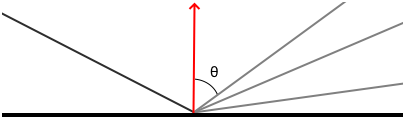
\includegraphics[scale=0.35]{rays.png}
\caption{incoming and outgoing rays}
\label{fig:incoming and outgoing rays}
\end{figure}

\section{BRDF (bidirectional reflective distribution function)}

The bidirectional reflective distribution function is a function that defines how light is reflected at an opaque surface. Physically realistic BRDFs have additional properties:

\begin{itemize}
  \item Positivity: $f_{r}\left (  p, w_{i}, w_{o} \right ) \geq 0$
  \item Obeying Helmholtz reciprocity: $f_{r}\left (  p, w_{i}, w_{o} \right ) = f_{r}\left (  p, w_{o}, w_{i} \right )$
  \item Conserving energy: $\forall \omega_{i} \int_{\Omega}f_{r}dw_{o} \leq 1$ the outgoing energy is never greater than the incoming energy except if the material emits light
\end{itemize}

\subsection{BRDF definition}
In phisically based rendering, $f_{r}$ is a BRDF which is usually a vector function which returns a color although in some cases it can be a scalar function which scales the incoming light. There are different BRDF, even you can model your own one. In this case, we are going to use the Cook-Torrance BRDF, which is one of the most used ones.

\subsection{Cook-Torrance}

It simulates how light behaves using two distinct approaches, distinguishing between diffuse reflection and specular reflection. The concept revolves around the simulated material reflecting a specific quantity of light in various directions (Lambert) and another portion in a specular manner, akin to a mirror. Consequently, the Cook-Torrance BRDF doesn't entirely substitute the previous model. Instead, we can precisely define the extent of radiance diffused and the amount reflected in a specular fashion, tailoring the simulation to the characteristics of the material in question. Thus the Cook-Torrance BRDF is defined as:

$$f_{r} = k_{d}f_{lambert} + k_{s}f_{cook-torrance}$$
\\
$f_{lambert}$ is the refracted light (diffuse; light penetrating and exiting the material ) and $f_{cook-torrance}$ is the reflected light (specular).\newline
$k_{d}$ and $k_{s}$ are the ratios or the amount of diffuse and specular light. Due to energy conservation $k_{d} + k_{s} \leq 1$
\\
\begin{lstlisting}[language=C++]
Vector3 kS = fresnelSchlick(max(halfwayVector.dot(wo), 0.0f), specular);
Vector3 kD = Vector3(1.0f, 1.0f, 1.0f) - kS;
// Multiply kD by the inverse metalness such that only non-metals
// have diffuse lighting, or a linear blend if partly metal (pure metals
// have no diffuse light).
kD *= (1.0f - material.metallic);
\end{lstlisting}

\subsubsection{Fresnel approximation and energy ratios}
The Fresnel equation describes the ratio of light that gets reflected over the light that gets refracted, which varies over the angle we're looking at a surface.
\\
We can approximate this equation using the Fresnel-Schlick approximation:

$$F_{Schlick} \left( h, v, F_{0}\right) = F_{0} + \left(1 - F_{0} \right)\left[ 1 - \left( h \cdot v\right)\right]^{5}$$
\\
As $cos\theta= h \cdot v = h \cdot \omega_{o}$ we can also define the Fresnel-Schlick approximation as:
$$F_{Schlick} \left( h, cos\theta \right) = F_{0} + \left(1 - F_{0} \right)\left[ 1 - cos\theta\right]^{5}$$
$F_{0}$ represents the base reflectivity of the surface, which we calculate using the indices of refraction:
\\
$$F_{0}=\left( \frac{\eta_{1} - \eta_{2}}{\eta_{1} + \eta_{2}} \right)^{2}$$
\\
Then, the $k_{d}$ and $k_{s}$ energy ratios can be defined as:\newline
\\
$$k_{s} = F_{Schlick}(h, w_{o}, F_{0}), \quad k_{s} \in \mathbf{R^3}$$
$$k_{d} = 1 - k_{s}, \quad k_{d} \in \mathbf{R^3}\newline$$
\\
Where $h$ is the halfway vector, $v$ is the direction of the viewer and $F_{0}$ is the surface's response at normal incidence at a 0 degree angle as if looking directly onto the surface.\newline
\\
$h = \frac{l + v}{||l + v||}$. In this case $h = \frac{w_{i} + w_{o}}{||w_{i} + w_{o}||}$\newline
\\
\textbf{Fresnel equation table}\newline
Some of the more common values listed below as taken from Naty Hoffman's course notes:\newline
\begin{center}
\begin{tabular}{ |c | c | c |}
\hline
 \textbf{Material} & \textbf{$F_{0}$ (Linear)} & \textbf{$F_{0}$ (sRGB)} \\ 
 \hline
 Water & (0.02, 0.02, 0.02) & (0.15, 0.15, 0.15) \\  
 Plastic / Glass (Low) & (0.03, 0.03, 0.03) & (0.21, 0.21, 0.21) \\      
 Plastic High & 	(0.05, 0.05, 0.05) & (0.24, 0.24, 0.24) \\  
 Glass (high) / Ruby & (0.08, 0.08, 0.08) & (0.31, 0.31, 0.31) \\  
 Diamond & 	(0.17, 0.17, 0.17) & (0.45, 0.45, 0.45) \\  
 Iron & (0.56, 0.57, 0.58) & (0.77, 0.78, 0.78) \\  
 Copper & (0.95, 0.64, 0.54)	& (0.98, 0.82, 0.76) \\  
 Gold & 	(1.00, 0.71, 0.29) & (1.00, 0.86, 0.57) \\  
 Aluminium & (0.91, 0.92, 0.92) & (0.96, 0.96, 0.97) \\  
 Silver & (0.95, 0.93, 0.88)	 & (0.98, 0.97, 0.95) \\  
 \hline
\end{tabular}
\end{center}

\subsubsection{Diffuse light}
Diffuse light is the refracted light. Light penetrating and exiting the material. It is basically the color of the material. (The division by $\pi$  is a convention that helps normalize the diffuse reflectance in the Lambertian model. It ensures that the amount of reflected light is consistent with the spherical distribution of incident light, taking into account the average fraction of light contributing to diffuse reflection on a surface).\newline
\\
$f_{lambert} = \frac{c}{\pi}$ where $c$ is the albedo or surface color.

\subsubsection{Specular light}
Specular light is the reflected light. Metal materials does not have diffuse lighting, only specular. So the more metal a material is, the reflected color tends to be similar to the incoming light, whereas the more plastic (dia-electric) it is, the reflected color tends to be the albedo color.

$$f_{cook-torrance} = \frac{DFG}{4\left( \omega_{o} \cdot n \right)\left( \omega_{i} \cdot n \right)}$$
\\
$D$ is the normal distribution function, $F$ is the Fresnel equation and $G$ is the geometry function.\newline
\\
\textbf{Normal distribution function}\newline
The normal distribution function $D$ statistically approximates the relative surface area of microfacets exactly aligned to the (halfway) vector $h$ according to the roughness of the matrial $\alpha$. We'll be using the Trowbridge-Reitz GGX:

$$D(n,h,\alpha) = \frac{\alpha^{2}}{\pi \left[ \left( n \cdot h \right)^{2} \left( \alpha^{2} - 1\right) + 1\right]^{2}}$$
\\
\textbf{Geometry function}\newline
The geometry function statistically approximates the relative surface area where its micro surface-details overshadow each other, causing light rays to be occluded.

$$G(n,\omega_{o}, k) = \frac{n \cdot \omega_{o}}{\left( n \cdot \omega_{o}\right) \left( 1 - k\right) + k}$$
\\
Where $k$ is a remapping of $\alpha$ based on whether we're using the geometry function for either direct lighting or IBL lighting. $k_{direct} = \frac{\left( \alpha + 1\right)^{2}}{8}$ or $k_{IBL} = \frac{\alpha^{2}}{2}$. \newline
\\
To effectively approximate the geometry we need to take account of both the view direction (geometry obstruction) and the light direction vector (geometry shadowing). We can take both into account using Smith's method:

$$G(n,\omega_{o}, \omega_{i}, k) = G(n, \omega_{o}, k)G(n, \omega_{i}, k)$$

\subsection{Energy absorption}

Depending on the material with which the ray intersects, it absorbs more or less energy. So there is a new parameter for each material called absorption that will allow us to scale the radiance.

\begin{lstlisting}[language=C++]
Vector3 kS = fresnelSchlick(max(halfwayVector.dot(wo), 0.0f), specular);
Vector3 kD = Vector3(1.0f, 1.0f, 1.0f) - kS;
kD *= (1.0f - material.metallic);

float energyAbsorption = 1.0f - material.absorption
Vector3 fr = (kD.elementWiseProduct(diffuse) + specular) * energyAbsorption
\end{lstlisting}

\section{Final equation}
With every component of the Cook-Torrance BRDF described, we can include the physically based BRDF into the now final reflectance equation. Substituting $f_{r} = k_{d}f_{lambert} + k_{s}f_{cook-torrance}$ we get:

$$L_{o} \left (  p, w_{o} \right ) = L_{e} \left (  p, w_{o} \right ) + \int_{\Omega} \left[  k_{d}\frac{c}{\pi} + k_{s}\frac{DFG}{4\left( \omega_{o} \cdot n \right)\left( \omega_{i} \cdot n \right)} \right] L_{i} \left (  p, w_{i} \right ) (w_{i} \cdot n) dw_{i}$$
\\
This equation is not fully mathematically correct however. You may remember that the Fresnel term $F$ represents the ratio of light that gets reflected on a surface. This is effectively our ratio $k_{s}$, meaning the specular (BRDF) part of the reflectance equation implicitly contains the reflectance ratio $k_{s}$. Given this, our final final reflectance equation becomes:

$$L_{o} \left (  p, w_{o} \right ) = L_{e} \left (  p, w_{o} \right ) + \int_{\Omega} \left[  k_{d}\frac{c}{\pi} + \frac{DFG}{4\left( \omega_{o} \cdot n \right)\left( \omega_{i} \cdot n \right)} \right] L_{i} \left (  p, w_{i} \right ) (w_{i} \cdot n) dw_{i}$$
\\
Solving the previous equation using Monte Carlo and the Cook Torrance BRDF we get the following estimator:
$$\hat{L}_{o}\left (  p, w_{o} \right ) = L_{e} \left (  p, w_{o} \right ) + \frac{2\pi}{N}\sum_{i=0}^{N}\left[  k_{d}\frac{c}{\pi} + \frac{DFG}{4\left( \omega_{o} \cdot n \right)\left( \omega_{i} \cdot n \right)} \right]L_{i} \left (  p, w_{i} \right ) \left ( w_{i} \cdot n \right )$$

\section{Algorithm overview}

\begin{itemize}
  \item For each pixel throw a ray from the camera.
  \item If it intersects nothing, $L{o} = (0,0,0)$ or $L{o} = \text{sky color}$
  \item If it intersects with an object. Solve the rendering equation using the Monte Carlo estimator. For each intersection, throw N rays (their direction depend on the roughness of the material intersected). And for each ray, solve the rendering equation. Keep in mind that $L_{o}^{t+1} = L_{i}^{t}$. It is a recursive problem that iterates a number of bounces.
  \item The recursive equation would look like this (It is the same as the recursive integral equation defined in page 1, but now using Monte Carlo in order to solve those integrals):
  $$\hat{L}_{o1} = L_{e1} + \frac{2\pi}{N}\sum_{i=0}^{N}f_{r1}L_{i1} \left ( w_{i1} \cdot n_{1} \right ) =  L_{e1} + \frac{2\pi}{N}\sum_{i=0}^{N}f_{r1} \left(  L_{e2} + \frac{2\pi}{N}\sum_{i=0}^{N}f_{r2}L_{i2} \left ( w_{i2} \cdot n_{2} \right ) \right) \left ( w_{i1} \cdot n_{1} \right )=$$

  $$=L_{e1} + \frac{2\pi}{N}\sum_{i=0}^{N}f_{r1} \left[  L_{e2} + \frac{2\pi}{N}\sum_{i=0}^{N}f_{r2} \left( L_{e3} + \frac{2\pi}{N }\sum_{i=0}^{N}f_{r3} \cdot \cdot \cdot \left ( w_{i3} \cdot n_{3} \right ) \right) \left ( w_{i2} \cdot n_{2} \right ) \right] \left ( w_{i1} \cdot n_{1} \right )$$
  \item Consider bidirectional path tracing in order to get better results. Some times, depending on the environment, reaching a light is quite difficult, so that all the scene would be much darker (or even completely black) than it should be. So one way to solve this is not only throwing rays from the camera, but also from the light source and joining them in the same path. 
\end{itemize}

\section{Ray tracing and global illumination approach}
There are points in the scene that are directly illuminated, that is, there is no object between the light source and the point. So we know with certainty, that point will be illuminated by that light source. However, using pure path tracing implies that some rays with random directions may not reach the light source, obtaining noisy results.\newline
In order to solve this, it is possible to compute the direct and indirect lighting and combine them together. 

\begin{itemize}
  \item Direct lighting: throw a ray from the point to each light source in the scene. Consider the light source if the ray DOES NOT intersect with any other object in the scene, that is, that the point is directly illuminated by that light source.
  Thus, each $L_i$ is nothing but each light source that contributes directly to the illumination of the point.
  $$L_{dl} \left (  p, w_{o} \right ) = L_{e} \left (  p, w_{o} \right ) + \int_{\Omega} f_{r}\left (  p, w_{i}, w_{o} \right ) L_{i} w_{i} \cdot n dw_{i}$$
  \item Indirect lighting: to compute the indirect lighting just solve recursively the rendering equation as we do in pure path tracing:
  $$L_{il} \left (  p, w_{o} \right ) = L_{e} \left (  p, w_{o} \right ) + \int_{\Omega} f_{r}\left (  p, w_{i}, w_{o} \right ) L_{i} \left (  p, w_{i} \right ) \left(w_{i} \cdot n \right) dw_{i}$$
  \item Total lighting: the total lighting is nothing but the sum of direct and indirect lighting:
  $$L_T = L_{dl} + L_{il}$$
\end{itemize}

\section{Conclusions}

Monte Carlo path tracing is noisy. Using many samples and bounces will make the image look smoother but it will take much computational time.
\\
A good choice would be to denoise the image after generating it, this way there is no need on generating that many rays.
\\
Another choice would be using the ray tracing and global illumination approach, even if it is not as realistic as the pure path tracing approach, it is less noisy and has a better performance (it can be rendered in real time).

\section{Result}

\begin{figure}[h]
\centering
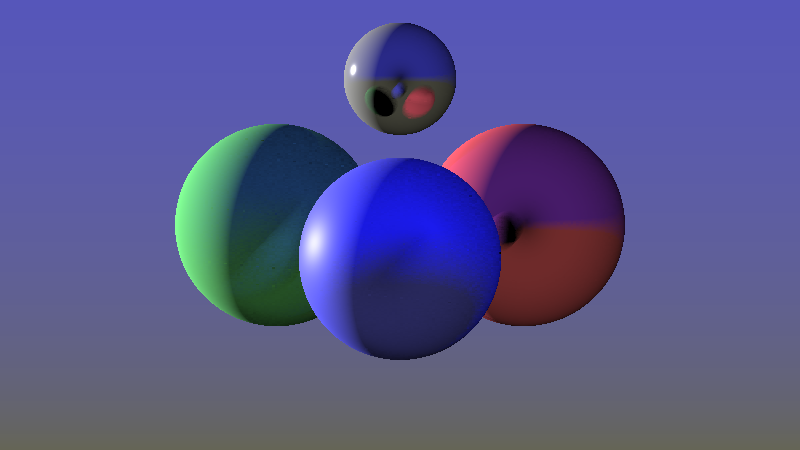
\includegraphics[scale=0.5]{raytracingGI.png}
\caption{Ray tracing and global illumination}
\label{fig:Ray tracing and global illumination}
\end{figure}

\end{document}